%%%%%%%%%%%%%%%%%%%
% SECTION: ANN
%%%%%%%%%%%%%%%%%%%
\section{Artificial Neural Networks}

The origin of an \textbf{Artificial Neural Network (ANN)} started when people tried to replicate the human neurons. Back in 1943, McCulloch and Pitts \cite{Mcculloch1990AACTIVITY} made the first contribution to ANN. They both tried to learn how the brain can compute complex behaviours using simple units such as the neurons. They designed a simple neuron using weighted inputs and one output that would seek to replicate such behaviour. Later, in 1958, Rosenblatt \cite{RosenblattTHEBRAIN} developed the \textbf{perceptron}.  This algorithm \ref{eq:perceptron} was a binary classifier that mapped a real value into a binary output.

\begin{equation} \label{eq:perceptron}
  f(x) = \left\{
  \begin{matrix}
    1 & if \quad w \cdot x + b > 0 \\ 
    0 & otherwise
  \end{matrix}
  \right.
\end{equation}

\subsection{Backpropagation and Stochastic Gradient Descent}

In 1985, Hinton and Williams \cite{Rumelhart1986LearningPropagation} rediscovered the backpropagation algorithm that was first introduced by Werbos \cite{Werbos1974BeyondSciences} in 1974. Backpropagation makes a forward pass of the input, when the input reaches the last layer, the prediction is compared to the ground truth. Using a loss function an error is calculated. The loss is then used to find the best gradient for minimizing the error using a partial derivative. This gradient is then used to update the weights of the last layer. Backpropagation uses the chain rule to compute the derivative of the previous layers and update the weights of all layers.

The first proposal used \textbf{Stochastic Gradient Descent (SGD)}. This method estimates the best direction for optimizing the function using only a random subset of the dataset. The backpropagation method is used iteratively until it ultimately fits the weights of all layers. Nowadays there exists more alternatives to SGD, these methods are called \textbf{Adaptative Learning Methods}. 

\subsection{Architecture of Neural Network}

A typical \textbf{Neural Network (NN)} has a huge number of artificial neurons, also called units, organised in different layers \cite{ArtificialApplications}. An ANN can be viewed as weighted directed graph in which \textbf{artificial neurons} are nodes, and directed edges with weights are connections between neuron outputs and neuron inputs.

The ANN receives information from the external world in the form of pattern and image in vector form. These inputs are mathematically designated by the notation $x(n)$ for n number of inputs.

Each input is multiplied by its corresponding weights. Weights are the information used by the neural network to solve a problem. Typically weight represents the strength of the interconnection between neurons inside the neural network.

% Layers
\subsubsection{Layers}

The simplest form of an ANN is the \textbf{Feed-Forward Neural Network}. 
In this kind of network, nodes are arranged in layers. Nodes from the adjacent layers have connections among them. These connections represent the weights between layers of nodes. In a feed-forward neural network, there are three different kind of layers:
\begin{itemize}
	\item 
Input layer: It contains those units (artificial neurons) which receive input from the outside world on which network will learn, recognize about or otherwise process.
	\item 
Hidden layer: These units are in between input and output layers. The job of hidden layer is to transform the input into something that output unit can use in some way.
	\item 
Output layer: It contains units that respond to the information about how it’s learned any task.
\end{itemize}

% FIGURE: ANN Architecture
\begin{figure}[!htb]	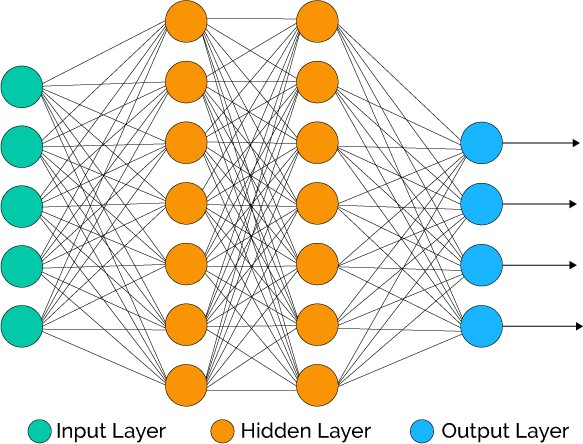
\includegraphics[width=0.7\textwidth]{images/architecture_ann.jpg} 
    \centering

\caption{
Typical architecture of an Artificial Neural Network.\cite{ArtificialApplications}
} 

\label{fig:architecture_ann}
\end{figure}

% Neurons
\subsubsection{Neurons}

The input value that neuron $k$ in layer $l$ receives is shown in equation \ref{eq:nueron-input}. Where $b_{k}^{l}$ is the bias in neuron $k$ in layer $l$. $N_{l-1}$ is the number of neurons in layer $l -1$. $w_{ik}^{l-1}$ is the weight that connects unit $i$ in layer $l -1$ and unit $k$ in layer $l$. $y_{i}^{l-1}$ is the output of unit $i$ in layer $l -1$. \cite{Krizhevsky2009LearningImages}

\begin{equation} \label{eq:nueron-input}
	x_{k}^{l}= b_{k}^{l} \sum_{i=1}^{N_{l-1}} w_{ik}^{l-1} y_{i}^{l-1}
\end{equation}

The output value that a neuron computes in a hidden layer is shown in equation \ref{eq:nueron-output}. Where $f$ is a differentiable function of the total inputs of the neuron.

\begin{equation} \label{eq:nueron-output}
	y_{k}^{l} = f(x_{k}^{l})
\end{equation}

Figure \ref{fig:single_neuron} represents the schema of a single neuron function $f(x_{k}^{l})$ with inputs $x_{k}^{l}$, biases $b_{k}^{l}$ and output $y_{k}^{l}$.

% FIGURE: ANN Architecture
\begin{figure}[!htb]	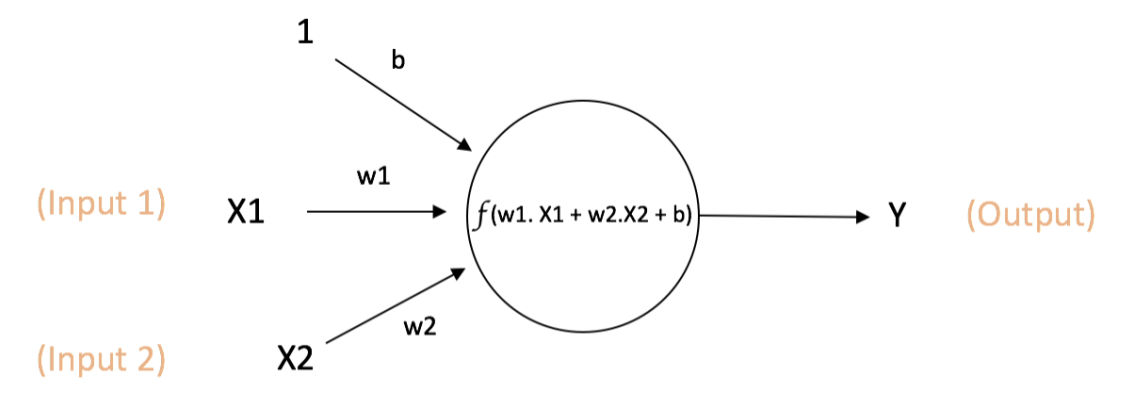
\includegraphics[width=0.7\textwidth]{images/single_neuron.png} 
    \centering

\caption{
A single neuron schema.\cite{ABlog}
} 

\label{fig:single_neuron}
\end{figure}